\chapter{Teoria da Integração}
Uma vez que já foram bem explorados os espaços mensuráveis e os espaços de medida, vamos abordar, nesta seção, a teoria da integração de Lebesgue.
Iniciaremos por funções não negativas e iremos estendendo os conceitos aos poucos.
Quando não houver menção contrária, $(X, \cc, \mu)$ será um espaço de medida.
O conjunto de todas as funções $f:X \to \xreta$ mensuráveis será simplesmente denotado por $M = M(X, \cc)$ e o conjunto das funções não negativas, que também são $\cc$-mensuráveis será denotado por $M^+ = M^+(X, \cc)$. 

\section{A Integral de Funções Simples}
	Iniciaremos tratando de casos particulares de integral e depois vamos expandindo.
	Com isso, iniciaremos entendo a integral para funções simples.

\begin{env}{Definição}
    Uma função real é dita simples quando possui apenas uma quantidade finita de valores.
\end{env}

Representaremos esse tipo de função de forma padronizada em todo o texto.
Faremos isso por meio da seguinte forma
$$
\varphi =  \sum_{j = 1}^n a_j\chi_{E_j}
$$
onde $a_j \in \R$ e $\chi_{E_j}$ é a função característica do conjunto $E_j \in \cc$.
Nessa representação estamos supondo que cada $a_j \neq a_i$ quando $j \neq i$ e que
$\displaystyle \bigcup_{j = 1}^n E_j = X$ onde a sequência finita de conjuntos $(E_n)$ formam uma partição do conjunto $X$.

\begin{env}{Exemplo}
\label{ex:função-escada-part-2}

    Seja $g: [0,4] \to \R$ pondo 
    
    $$g(x) = \left\{
    \begin{array}{cc}
         1, & \textrm{\ se } x \in [0,1] \\
         2, & \textrm{\ se } x \in [1,2) \\
         3, & \textrm{\ se } x \in [2,3) \\
         4, & \textrm{\ se } x \in [3,4]
    \end{array}\right.
    $$
    Claramente, $g$ também é uma função simples.
    Basta denotar 
    $E_1 = [0,1),\ 
     E_2 = [1,2),\   
     E_3 = [2,3),\  
     E_4 = [3,4]$ e 
     $ a_i = i$ para $1 \leq i \leq 4$.
    Com isso, vemos que para $x \in [0,4]$
    $$
    g(x) = 1\cdot \chi_{[0,1]}(x) + 2\cdot \chi_{(1,2]}(x) + 3\cdot \chi_{(2,3]}(x) + 4\cdot \chi_{(3,4]}(x)
    $$
    Concluindo que $g = \dsum_{j = 1}^4 a_j\chi_{E_j}$. 
\end{env}

  
    \begin{figure}[h!]
	\centering
	\Caption{\label{fig:gráfico-função-simples-g-sobre-[0,4]} Gráfico da Função $g =\dsum_{j = 1}^4 a_j\chi_{E_j}$}	
	\UECEfig{}{
	    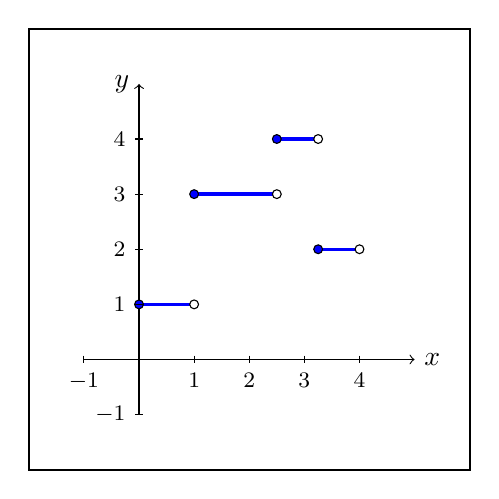
\begin{tikzpicture}[scale=0.7]
				
				\draw[thick] (-2,-2) rectangle (6, 6);
                % Eixos
                \draw[->] (-1,0) -- (5,0) node[right] {$x$};
                \draw[->] (0,-1) -- (0, 5) node[left] {$y$};
                                
                % Plot do gráfico
                \draw[domain=0:1,very thick,variable=\x,blue] plot ({\x},{1});
                \draw[domain=1:2.5,very thick,variable=\x,blue] plot ({\x},{3});
                \draw[domain=2.5:3.25,very thick,variable=\x,blue] plot ({\x},{4});
                \draw[domain=3.25:4,very thick,variable=\x,blue] plot ({\x},{2});
        		
        		% Bolinhas dos Intervalos
        		\draw[fill=blue] (0,1) circle (0.08);
        		\draw[fill=blue] (1,3) circle (0.08);
        		\draw[fill=blue] (2.5,4) circle (0.08);
        		\draw[fill=blue] (3.25,2) circle (0.08);
        		
        		\draw[fill=white] (1,1) circle (0.08);
        		\draw[fill=white] (2.5,3) circle (0.08);
        		\draw[fill=white] (3.25,4) circle (0.08);
        		\draw[fill=white] (4,2) circle (0.08);
        		                

                % Rótulos
                \foreach \i in {-1,1,2,3,4}{
                \draw (\i,2pt)--(\i, -2pt) node[below]{{\footnotesize $\i$}};
                }
                
                \foreach \i in {-1,1,2,3,4}{
                \draw (2pt,\i)--(-2pt, \i) node[left]{{\footnotesize $\i$}};
                }
                
                % Linhas trastejadas
                % \foreach \i in {1,2,3,4}{
                % \draw[dashed, help lines] (\i,0) -- (\i,\i);
                % }
                % \foreach \i in {1,2,3}{
                % \draw[dashed, help lines] (\i,\i) -- (\i,\i+1);
                % }  
            \end{tikzpicture}
	}{
	    \Fonte{Elaborado pelo autor}
	}	
    \end{figure} 
Agora pensemos na ideia de integral apresentada na disciplina de Cálculo Diferencial e Integral.
Se quiséssemos calcular a integral das funções acima somaríamos as áreas dos retângulos conforme ilustram as figuras a seguir.\\
 
    %Gráfico da função g
    \begin{figure}[!h]
	\centering
	\Caption{\label{fig:integral-função-simples-g-sobre-[0,4]} Área delimitada pelo gráfico da função $g =\dsum_{j = 1}^4 a_j\chi_{E_j}$}	
	\UECEfig{}{
	    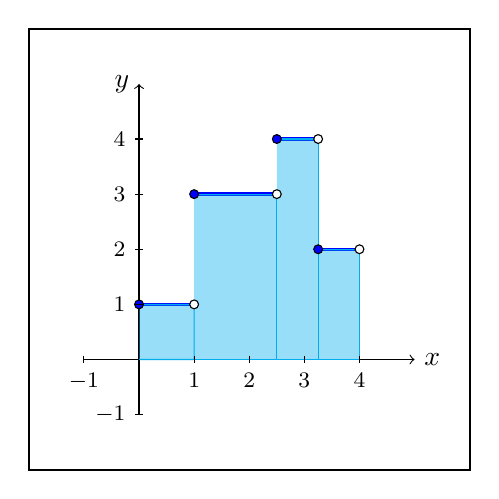
\begin{tikzpicture}[scale=0.7]
	    	\draw[thick] (-2,-2) rectangle (6, 6);
                % Eixos
                \draw[->] (-1,0) -- (5,0) node[right] {$x$};
                \draw[->] (0,-1) -- (0, 5) node[left] {$y$};
                                
                % Plot do gráfico	
				\draw[domain=0:1,very thick,variable=\x,blue] plot ({\x},{1});
				\draw[domain=1:2.5,very thick,variable=\x,blue] plot ({\x},{3});
				\draw[domain=2.5:3.25,very thick,variable=\x,blue] plot ({\x},{4});
				\draw[domain=3.25:4,very thick,variable=\x,blue] plot ({\x},{2});

				
				\filldraw [domain=0:1,smooth,variable=\x, cyan, fill opacity=0.4]  plot ({\x},{1})--(1,0)--(0,0);
	            \filldraw [domain=1:2.5,smooth,variable=\x, cyan, fill opacity=0.4]  plot ({\x},{3})--(2.5,0)--(1,0);
				\filldraw [domain=2.5:3.25,smooth,variable=\x, cyan, fill opacity=0.4]  plot ({\x},{4})--(3.25,0)--(2.5,0);
				\filldraw [domain=3.25:4,smooth,variable=\x, cyan, fill opacity=0.4]  plot ({\x},{2})--(4,0)--(3.25,0);
                
        		% Bolinhas dos Intervalos
				\draw[fill=blue] (0,1) circle (0.08);
				\draw[fill=blue] (1,3) circle (0.08);
				\draw[fill=blue] (2.5,4) circle (0.08);
				\draw[fill=blue] (3.25,2) circle (0.08);
				
				\draw[fill=white] (1,1) circle (0.08);
				\draw[fill=white] (2.5,3) circle (0.08);
				\draw[fill=white] (3.25,4) circle (0.08);
				\draw[fill=white] (4,2) circle (0.08);


                % Rótulos
                \foreach \i in {-1,1,2,3,4}{
                \draw (\i,2pt)--(\i, -2pt) node[below]{{\footnotesize $\i$}};
                }
                
                \foreach \i in {-1,1,2,3,4}{
                \draw (2pt,\i)--(-2pt, \i) node[left]{{\footnotesize $\i$}};
                }
                
                % Linhas trastejadas
                % \foreach \i in {1,2,3,4}{
                % \draw[dashed, help lines] (\i,0) -- (\i,\i);
                % }
                % \foreach \i in {1,2,3}{
                % \draw[dashed, help lines] (\i,\i) -- (\i,\i+1);
                % }  
            \end{tikzpicture}
	}{
	    \Fonte{Elaborado pelo autor}
	}	
    \end{figure} 
Note que em ambos os casos estamos, basicamente, aplicando o valor $a_j$ na medida do conjunto $E_j$ correspondente onde $j$ é o número de partições do domínio. Com isso, temos a definição a seguir:
\begin{env}{Definição}
\label{def:integral-função-naonegativa-simples}
    Se $\varphi$ é uma função simples de $M^+(X, \cc)$ com a representação 
    $$\varphi =  \sum_{j = 1}^n a_j\chi_{E_j},$$ então a integral da função $\varphi$ com respeito à medida $\mu$ é o valor real estendido
    $$
    \int\varphi d\mu = \sum_{j = 1}^n a_j\mu(E_j).
    $$
\end{env}

Para a \ref{def:integral-função-naonegativa-simples} empregamos a convenção que $0 \cdot (+\infty) = 0$.
Isso é feito para garantir que a função identicamente nula tenha integral nula independentemente da medida ser finita ou não.
A seguir veremos propriedades elementares sobre a integral de funções simples.

\begin{comment}
	

Antes disso, considere um espaço de medida $(X, \cc, \mu)$.
Seja  $\{E_n\}$ uma partição de $X$ com $n \in I_5$ conforme a representação a seguir.\pagebreak
\begin{figure}[h]
	\centering
	\Caption{\label{fig:particao-E-de-X} Partição $\{E_n\}$ do conjunto $X$} 
	\UECEfig{}{
		% Partição de X por E_n
		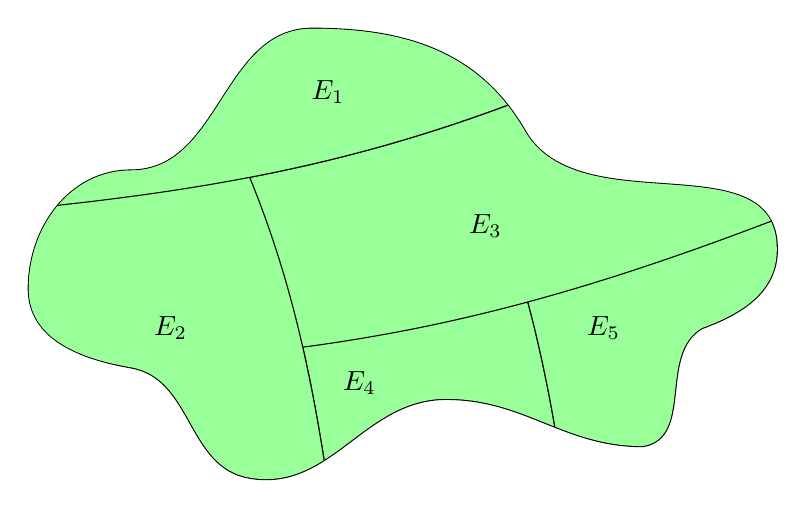
\begin{tikzpicture}
			% Define coordenadas que serão utilizadas posteriormente
			\path
			coordinate (aux0) at (0,1.5)
			coordinate (aux1) at (0,3.5)
			coordinate (aux2) at (10,3.5)
			coordinate (aux3) at (9,6)
			coordinate (aux4) at (4,0)
			coordinate (aux5) at (7,0)
			coordinate (aux6) at (2,6)
			coordinate (aux7) at (5,6)
			coordinate (esp1) at (0.2,2.5)
			coordinate (esp2) at (1.5,1.5)
			coordinate (esp3) at (3,0.1)
			coordinate (esp4) at (5.5,1.1)
			coordinate (esp5) at (8,0.5)
			coordinate (esp6) at (8.75,2)
			coordinate (esp7) at (9.7,3)
			coordinate (esp8) at (6.5,4.5)
			coordinate (esp9) at (3.8,5.8)
			coordinate (esp10) at (1.5,4)
			coordinate (nome) at (0, 6)
			;
			% Desenha curvas com angulação de saida e entrada
			\draw[line width=0.8pt]
			(esp1) to[out=-90,in=170]
			(esp2) to[out=-10,in=170]
			(esp3) to[out=-10,in=180]
			(esp4) to[out=0,in=180]
			(esp5) to[out=10,in=-150]
			(esp6) to[out=20,in=-90]
			(esp7) to[out=90,in=-60]
			(esp8) to[out=120,in=0]
			(esp9) to[out=180,in=0]
			(esp10) to[out=180,in=90]
			cycle;    
			% Limita a figura às coordenadas citadas
			\clip
			(esp1) to[out=-90,in=170]
			(esp2) to[out=-10,in=170]
			(esp3) to[out=-10,in=180]
			(esp4) to[out=0,in=180]
			(esp5) to[out=10,in=-150]
			(esp6) to[out=20,in=-90]
			(esp7) to[out=90,in=-60]
			(esp8) to[out=120,in=0]
			(esp9) to[out=180,in=0]
			(esp10) to[out=180,in=90]
			cycle;    
			
			\draw[fill=green!40]
			(aux4) to[bend right=10]
			(aux6) --
			(aux7) to[bend left=10]
			(aux5) -- cycle;
			\draw[fill=green!40]
			(aux5) to[bend right=10]
			(aux7) --
			(10,6) --
			(10,0) -- cycle;
			\draw[fill=green!40]
			(aux0) -- 
			(aux1) to[bend right=10]
			(aux3) --
			(10,6) -- 
			(aux2) to[bend left=10] cycle;
			\draw[fill=green!40]
			(0,0) -- 
			(aux4) to[bend right=10]
			(aux6) --
			(0,6) -- 
			(0,0) -- cycle;
			\draw[fill=green!40]
			(0,6) -- 
			(aux1) to[bend right=10]
			(aux3) --
			(0,6) -- cycle;
			\node at (4,5) {$E_1$};  
			\node at (2,2) {$E_2$};  
			\node at (6,3.3) {$E_3$};  
			\node at (4.4,1.3) {$E_4$};  
			\node at (7.5,2) {$E_5$};
			\node at (0.1,5.5) {$X$};  
			
		\end{tikzpicture}
		
	}{
		\Fonte{Elaborado pelo autor}
	}   
\end{figure}

\hspace{-2cm}Tome também uma outra partição $\{F_m\}$ onde $m \in I_6$.\\

\begin{figure}[h!]
	\centering
	\Caption{\label{fig:particao-F-de-X} Partição $\{F_m\}$ do conjunto $X$} 
	\UECEfig{}{
		% Partição F_m
		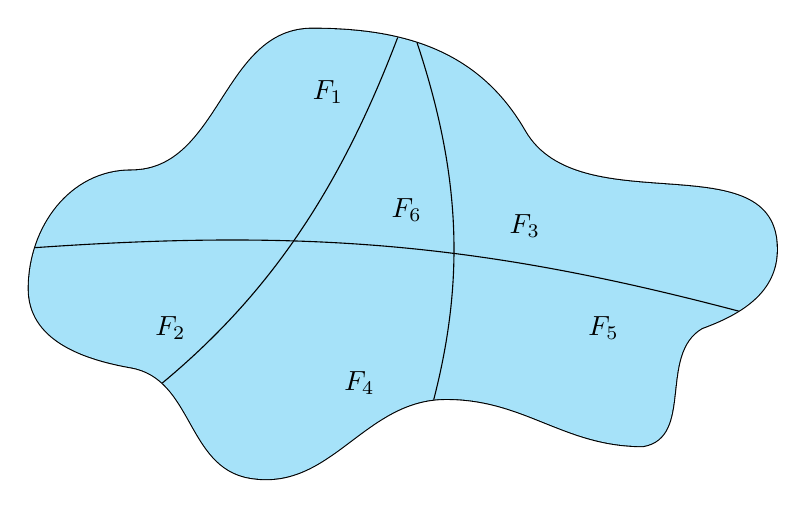
\begin{tikzpicture}
			% Define coordenadas que serão utilizadas posteriormente
			\path
			coordinate (aux0) at (1.1,2)
			coordinate (aux1) at (0,3.5)
			coordinate (aux2) at (10,3.5)
			coordinate (aux3) at (9,6)
			coordinate (aux4) at (4,0)
			coordinate (aux5) at (7,0)
			coordinate (aux6) at (2,6)
			coordinate (aux7) at (5,6)
			coordinate (aux8) at (11,2)
			coordinate (aux9) at (3,8.2)
			coordinate (esp1) at (0.2,2.5)
			coordinate (esp2) at (1.5,1.5)
			coordinate (esp3) at (3,0.1)
			coordinate (esp4) at (5.5,1.1)
			coordinate (esp5) at (8,0.5)
			coordinate (esp6) at (8.75,2)
			coordinate (esp7) at (9.7,3)
			coordinate (esp8) at (6.5,4.5)
			coordinate (esp9) at (3.8,5.8)
			coordinate (esp10) at (1.5,4)
			coordinate (nome) at (0, 6)
			;
			% Desenha curvas com angulação de saida e entrada
			\draw[line width=0.8pt]
			(esp1) to[out=-90,in=170]
			(esp2) to[out=-10,in=170]
			(esp3) to[out=-10,in=180]
			(esp4) to[out=0,in=180]
			(esp5) to[out=10,in=-150]
			(esp6) to[out=20,in=-90]
			(esp7) to[out=90,in=-60]
			(esp8) to[out=120,in=0]
			(esp9) to[out=180,in=0]
			(esp10) to[out=180,in=90]
			cycle;    
			% Limita a figura às coordenadas citadas
			\clip
			(esp1) to[out=-90,in=170]
			(esp2) to[out=-10,in=170]
			(esp3) to[out=-10,in=180]
			(esp4) to[out=0,in=180]
			(esp5) to[out=10,in=-150]
			(esp6) to[out=20,in=-90]
			(esp7) to[out=90,in=-60]
			(esp8) to[out=120,in=0]
			(esp9) to[out=180,in=0]
			(esp10) to[out=180,in=90]
			cycle;    
			
			\draw[fill=cyan!35] 
			(0,0) rectangle (10,6);
			\draw
			(0,0) 
			to[bend right = 20] 
			(aux7)
			to[bend right = 22] 
			(aux1);
			\draw
			(0,3) 
			to[bend left = 10] 
			(10,2)
			to[bend right = 10]
			(5,-6);
			\draw
			(5,0) 
			to[bend right = 20] 
			(aux7)
			to[bend right = 22] 
			(aux1);
			
			
			% Rótulos
			\node at (4,5) {$F_1$};  
			\node at (2,2) {$F_2$};  
			\node at (6.5,3.3) {$F_3$};  
			\node at (4.4,1.3) {$F_4$};  
			\node at (7.5,2) {$F_5$};  
			\node at (5,3.5) {$F_6$};
		\end{tikzpicture}
		
	}{
		\Fonte{Elaborado pelo autor}
	}   
\end{figure}
Claramente, ao observar as figuras acima, podemos ver que $E_3$ possui interseção com $F_j$ para todo $j \in I_6$.
Assim, $E_5 = \displaystyle \bigcup_{j = 1}^6 (F_j\cap E_5)$ com $(F_j\cap E_5) = \varnothing,\ \forall j \in I_6$. 
Logo, 
$$
\mu(E_5) = \mu\left(\bigcup_{j = 1}^6 (F_j\cap E_5)\right)
= 
\sum_{j=1}^{6}\mu(F_j\cap E_5)
$$
A igualdade acima é valida mesmo se o conjunto em questão não tiver interseção com todos os outros da partição.
Neste caso, a interseção com os demais será vazia e soma associada à eles é 0.
Basta observar, por exemplo, o conjunto $E_1$ que tem interseção com $F_1, F_6$ e $F_3$, mas não se intersecta com $F_2, F_4$ e $F_5$.
Deste modo,
$$
\sum_{j=1}^{6}\mu(F_j\cap E_3)
= \mu(F_1\cap E_3) + \mu(F_6\cap E_3) + \mu(F_3\cap E_3)
= \mu(E_3)
$$
Pois, $\mu(F_2\cap E_3) = \mu(F_4\cap E_3) = \mu(F_5\cap E_3) = 0$.
\end{comment}

\begin{env}{Teorema}
	\label{teo:aritmetica-com-integrais-de-funções-simples}
    Se $\varphi$ e $\psi$ são funções simples do espaço $M^+(X,\cc)$ e $c\geq0$ é uma constante real, então
    $
    \displaystyle \int c\varphi d\mu = c \int \varphi d\mu
    $
	e
    $
    \displaystyle \int (\varphi + \psi) d\mu = \int \varphi d\mu + \int \psi d\mu.
    $
\end{env}
\begin{prova}
    Representaremos as funções simples não negativas por $\varphi = \dsum_{j = 1}^n a_j\chi_{E_j}$ e $\psi = \dsum_{k = 1}^m b_k\chi_{F_k}$.
    Primeiro, mostraremos que vale a multiplicação por escalar.
    Assim, caso $c = 0$, o resultado é verdadeiro trivialmente. 
    Supondo $c> 0$, temos que
    $$\int c \varphi\ d\mu = \dsum_{j = 1}^n c a_j\mu(E_j) = c \dsum_{j = 1}^n a_j\mu(E_j) = c\int \varphi \ d\mu.$$
    Com isso, concluímos que $\displaystyle \int c \varphi\ d\mu = c\int \varphi \ d\mu.$ 
    
    Dadas as representações padrão de $\varphi$ e $\psi$, vemos que
    
    \begin{equation}
    	\label{eq:somatorio funções simples}
    	\varphi +\psi
    	=
    	\dsum_{j = 1}^n a_j\chi_{E_j}
    	+
    	\dsum_{k = 1}^m b_k\chi_{F_k}
    \end{equation}
    
    Como $\{E_n\}$ e $\{F_k\}$ são ambas partições de $X$, pela \ref{prop: igualdade da caracteristica como medida} temos que
    $\chi_{E_j} = \dsum_{k = 1}^m \chi_{(E_j \cap F_k)}$ e 
    $\chi_{F_k} = \dsum_{j = 1}^n \chi_{(E_j \cap F_k)}$.
    Substituindo na equação \ref{eq:somatorio funções simples}, obtemos    
    \begin{align*}
    	\dsum_{j = 1}^n a_j\chi_{E_j}
    	+
    	\dsum_{k = 1}^m b_k\chi_{F_k}
    	= &
    	\dsum_{j = 1}^n a_j\left(\dsum_{k = 1}^m \chi_{(E_j \cap F_k)}\right)
    	+
    	\dsum_{k = 1}^m b_k\left(\dsum_{j = 1}^n \chi_{(E_j \cap F_k)}\right)\\
    	= &
    	\dsum_{j = 1}^n\dsum_{k = 1}^m a_j\chi_{(E_j \cap F_k)}
    	+
    	\dsum_{k = 1}^m \dsum_{j = 1}^n b_k\chi_{(E_j \cap F_k)}\\
    	= &
    	\dsum_{j = 1}^n\dsum_{k = 1}^m a_j\chi_{(E_j \cap F_k)}
    	+
    	\dsum_{j = 1}^n \dsum_{k = 1}^m  b_k\chi_{(E_j \cap F_k)}\\
		= &
		\dsum_{j = 1}^n\dsum_{k = 1}^m 
		\left(a_j\chi_{(E_j \cap F_k)}
		+
		b_k\chi_{(E_j \cap F_k)}\right)\\
		= &
		\dsum_{j = 1}^n\dsum_{k = 1}^m 
		(a_j + b_k)\chi_{(E_j \cap F_k)}.
	\end{align*}
    Com isso, concluímos que
    $$
    \varphi + \psi = \dsum_{j = 1}^n\dsum_{k = 1}^m(a_j + b_k)\chi_{E_j \cap F_k}.
    $$
    Entretanto, essa representação não é, necessariamente, a representação padrão apresentada na \ref{def:integral-função-naonegativa-simples}, pois 
    nada garante, previamente, que $a_j + b_k$ sejam distintos para $j \in I_n$ e $k \in I_m$.
    Com isso, sejam $c_h$, com $h \in I_p$, números distintos do conjunto $\{a_j + b_k; \ (j,k) \in I_n \times I_m\}$ e $G_h$ a união de todos os conjuntos $E_j \cap F_k \neq \varnothing$ tal que $a_j + b_k = c_h$.
    Assim, 
    $$
    G_h = \bigcup_{\begin{minipage}{1.4cm}
        \fontsize{8}{5}\selectfont
        \centering
        $j,k$
        $a_j + b_k = c_h$
    \end{minipage}} E_j \cap F_k
    $$
    A notação utilizada acima indica que a soma é realizada sobre todos os índices $j$ e $k$ tais que $a_j + b_k =c_h$.
    Como $E_j \cap F_k = \varnothing$, temos que 
    $$
    \mu(G_h) = \mu\left(\bigcup_{
        j,k\atop
        a_j + b_k = c_h} E_j \cap F_k
    \right)
    = 
    \sum_{
        j,k\atop
        a_j + b_k = c_h} \mu(E_j \cap F_k)
    $$
    Desta forma, conseguimos encontrar uma representação padrão que é dada por 
    $\displaystyle \varphi + \psi = \sum_{h =1}^p c_h\chi_{G_h}$.
    Logo, temos que 
    \begin{align*}
        \int(\varphi + \psi) d\mu = \sum_{h =1}^p c_h\mu(G_h)
        = & 
        \sum_{h = 1}^p\sum_{ j,k\atop a_j + b_k = c_h}c_h \mu(E_j \cap F_k)\\
        = &
        \sum_{h = 1}^p\sum_{ j,k\atop a_j + b_k = c_h}(a_j + b_k) \mu(E_j \cap F_k)\\
        = &
        \sum_{j = 1}^n\sum_{k = 1}^m(a_j + b_k) \mu(E_j \cap F_k)\\
        = &
        \sum_{j = 1}^n\sum_{k = 1}^m a_j \mu(E_j \cap F_k) + \sum_{j = 1}^n\sum_{k = 1}^m b_k \mu(E_j \cap F_k)
    \end{align*}
	Pela \ref{prop: medida com partição}, temos
	$
	\displaystyle
	\mu(E_j) = \sum_{k = 1}^m \mu(E_j \cap F_k)
	$
    e
    $\displaystyle \mu(F_k) = \sum_{j = 1}^n \mu(E_j \cap F_k)$.
    Empregando estes resultados ao que foi desenvolvido anteriormente obtemos
    $$
    \sum_{j = 1}^n\sum_{k = 1}^m a_j \mu(E_j \cap F_k) + \sum_{j = 1}^n\sum_{k = 1}^m b_k \mu(E_j \cap F_k)
    =
    \sum_{j = 1}^n a_j \mu(E_j) + \sum_{k = 1}^m b_k \mu(F_k)
    =
    \int \varphi d\mu + \int \psi d\mu
    $$
    Segue que $\displaystyle\int(\varphi + \psi) d\mu = \int \varphi d\mu + \int \psi d\mu$ como queríamos.
\end{prova}


% Lemas para o teorema

\begin{env}{Lema}
	\label{lem:medida-da-intersecao-de-um-fixado}
	Se $\mu$ é uma medida sobre $X$ e fixemos um elemento $A$ de $\cc$, então a função $\lambda$ definida por $\lambda(E) = \mu(A\cap E), \ \forall\  E \in \cc$ também é uma medida sobre $X$.
\end{env}
\begin{prova}
	Basta mostrar que $\lambda$ satisfaz as condições impostas na definição \ref{def:medida}.
	Com isso, se $E = \varnothing$, então
	$$
	\lambda(\varnothing) = \mu(A \cap \varnothing) = \mu(\varnothing) = 0
	$$
	Como $A$ e $E$ são elementos de $\cc$, então $A \cap H$ também está em $\cc$.
	Assim, por $\mu$ ser uma medida, temos que $\mu(A\cap E) \geq 0$ acarretando que $\lambda(E) \geq 0$.
	Por fim, tomemos uma sequência de elementos disjuntos $(E_n)$ em $\cc$.
	Se $A = E_j$ para algum $j \in \N$, não há o que fazer.
	Caso $A \cap E_j = \varnothing$ para qualquer que seja $j \in \N$, então $\displaystyle \left( \bigcup_{n \in \N} E_n\right) \cap A = \varnothing$.
	Com isso, 
	
	\begin{align*}
		\left( \bigcup_{n \in \N} E_n\right) \cap A
		= &
		(E_1 \cup E_2 \cup \cdots \cup E_n \cup \cdots) \cap A\\
		= &
		(E_1 \cap A )\cup (E_2 \cap A) \cup \cdots \cup (E_n\cap A) \cup \cdots \\
		= &
		\bigcup_{n \in \N} (E_n\cap A)    
	\end{align*}
	%   
	Segue então que
	$$
	\lambda\left( \bigcup_{n \in \N} E_n\right)
	=
	\mu\left(\left( \bigcup_{n \in \N} E_n\right) \cap A\right)
	=
	\mu\left( \bigcup_{n \in \N} (E_n\cap A) \right)
	=
	\sum_{j = 1}^\infty \mu(E_j \cap A)
	= 
	\sum_{j = 1}^\infty \lambda(E_j)
	$$
	Desta forma, concluímos que a função $\lambda$ acima definida é uma medida.
\end{prova}

\begin{env}{Lema}
	\label{lem:medida-gerada-por-medidas-e-numeros-reais}
	Se $\mu_1, ..., \mu_n$ são medidas sobre $X$ e $a_1, ... , a_n$ são números reais não negativos, então a função $\lambda$ definida por
	$\lambda(E) = \dsum_{j =1}^n a_j\mu_j(E), \forall\  E \in \cc$ também é uma medida sobre $X$.
\end{env}
\begin{prova}
	Como $\mu_j$ é uma medida para todo $j \in I_n$ e cada $a_j$ é maior ou igual à zero, temos que cada $a_j\mu_j(E) \geq 0$.
	Desta maneira, $\lambda(E) = \displaystyle \sum_{j = 1}^n a_j\mu_j(E) \geq 0$.
	Além disso, podemos observar que $\lambda(\varnothing) = \displaystyle \sum_{j =1}^n a_j\mu_j(\varnothing) = 0$.
	Tomemos uma sequência disjunta $(E_p)$ de elementos de $\cc$.
	Logo, 
	$$
	\lambda\left(\bigcup_{p \in \N} E_p\right)
	=
	\sum_{j = 1}^n a_j\mu_j\left(\bigcup_{p \in \N} E_p\right)
	=
	\sum_{j = 1}^n a_j\left(\sum_{p = 1}^\infty\mu_j(E_p)\right)
	=
	\sum_{p = 1}^\infty\left(\sum_{j = 1}^na_j\mu_j(E_p)\right)
	=
	\sum_{p = 1}^{\infty}\lambda(E_p)
	$$
	\begin{comment}
	Afirmamos que $\displaystyle \sum_{j = 1}^n a_j\left(\sum_{p = 1}^\infty\mu_j(E_p)\right) = \sum_{p = 1}^\infty\left(\sum_{j = 1}^na_j\mu_j(E_p)\right)$.
	Com efeito, 
	\begin{align*}
	\sum_{j = 1}^n a_j\left(\sum_{p = 1}^\infty\mu_j(E_p)\right)
	= &
	\sum_{j = 1}^n a_j\left(\lim_{m \to +\infty}\sum_{p = 1}^m\mu_j(E_p)\right)\\
	= &
	\lim_{m \to +\infty}\left[\sum_{j = 1}^n a_j\left(\sum_{p = 1}^m\mu_j(E_p)\right)\right]\\
	= &
	\lim_{m \to +\infty}\left[a_1\left(\sum_{p = 1}^m\mu_1(E_p)\right)+ \cdots + a_n\left(\sum_{p = 1}^m\mu_n(E_p)\right)\right]\\
	= &
	\lim_{m \to +\infty}\left(\sum_{p = 1}^ma_1\mu_1(E_p)+ \cdots + \sum_{p = 1}^ma_n\mu_n(E_p)\right)\\
	= &
	\lim_{m \to +\infty}\sum_{p = 1}^m \left(a_1\mu_1(E_p)+ \cdots + a_n\mu_n(E_p)\right)\\
	= &
	\lim_{m \to +\infty}\sum_{p = 1}^m \left(\sum_{j = 1}^na_j\mu_j(E_p)\right)\\
	= &
	\sum_{p = 1}^\infty \left(\sum_{j = 1}^na_j\mu_j(E_p)\right)\\
\end{align*}		
	\end{comment}
	
\begin{comment}
		Disso tudo, obtemos que 
	$$
	\lambda\left(\bigcup_{p \in \N} E_p\right)
	=
	\sum_{j = 1}^n a_j\left(\sum_{p = 1}^\infty\mu_j(E_p)\right)
	=
	\sum_{p = 1}^\infty \left(\sum_{j = 1}^na_j\mu_j(E_p)\right)
	=
	\sum_{p = 1}^\infty \lambda(E_p)
	$$
\end{comment}

	Como $\lambda$ satisfaz todas as condições impostas na definição \ref{def:medida} concluímos que $\lambda$ é uma medida.    
\end{prova}

\begin{env}{Teorema}
	\label{teo:medida-atraves-de-uma-integral}
	A função $\lambda: \cc \to \xreta$ definida por
	$
	\displaystyle\lambda(E) = \int \varphi\chi_E\ d\mu
	$
	para todo $E \in \cc$ é uma medida sobre $\cc$. 
\end{env}

\begin{prova}
	De maneira análoga ao teorema \ref{teo:aritmetica-com-integrais-de-funções-simples}
	podemos verificar que 
	$$
	\varphi\chi_E = \sum_{j = 1}^n a_j\chi_{E_j \cap E}
	$$
	Assim, temos que 
	\begin{align*}
		\lambda(E) 
		= \int \varphi\chi_E d\mu
		= \int\left(\sum_{j = 1}^n a_j\chi_{E_j \cap E}\right)d\mu
		= \sum_{j = 1}^n\left(a_j\int \chi_{E_j \cap E}d\mu\right) 
		= \sum_{j = 1}^n a_j\mu(E_j\cap E)
	\end{align*}
	Pelo lema \ref{lem:medida-da-intersecao-de-um-fixado} a aplicação que leva 
	$E \to \mu(E_j\cap E)$ é uma medida para cada $j \in I_n$.
	Disso, concluímos que $\lambda$ pode ser expressada por uma combinação linear de medidas sobre $\cc$.
	Segue, pelo lema \ref{lem:medida-gerada-por-medidas-e-numeros-reais}, que 
	$\lambda$ também é uma medida sobre $\cc$.
\end{prova}

% Mostrar que existe uma função simples que aproxima uma função
\section{A Integral de Funções Não-Negativas}

Até aqui trabalhos apenas com integrais de funções simples apenas.
Nesta seção, desejamos expandir o conceito de integral para uma função qualquer não negativa.
Vale ressaltar que a perspectiva que traremos aqui é a de Lebesgue.
Com o intuito de enfatizar a diferença da construção, vamos lembrar da construção feita por Riemann.
Considere a função $f: \R \to \R$ tal que $f(x) = \mathrm{sen}(x) + 3$.
Claramente não é uma função simples, pois não possui uma quantidade finita de valores. 
Nosso objetivo, agora, é tentar calcular a integral dessa função com o que construímos até aqui.
Para facilitar, observe o gráfico dessa função no intervalo $[0,4]$ apresentado na figura \ref{fig:gráfico da função sen x + 3}.

\begin{figure}[h!]
	\centering
	\Caption{\label{fig:gráfico da função sen x + 3} Gráfico da função $f(x) = \textrm{sen}(x) + 3$} 
	\UECEfig{}{
		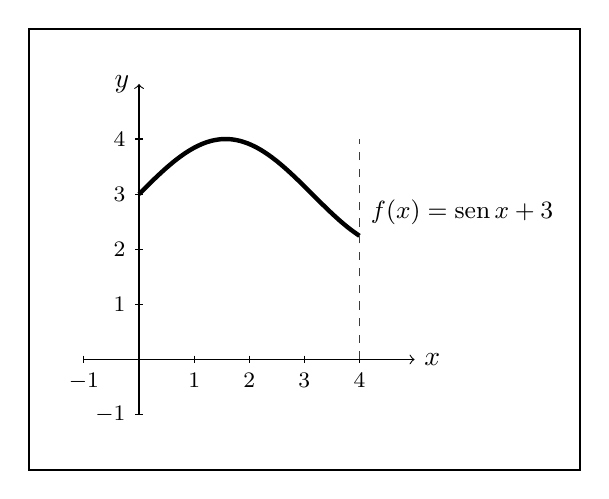
\begin{tikzpicture}[scale=0.7]
			\draw[thick] (-2,-2) rectangle (8, 6);
			% Eixos
			\draw[->] (-1,0) -- (5,0) node[right] {$x$};
			\draw[->] (0,-1) -- (0, 5) node[left] {$y$};
			
			% Plot do gráfico
			%	\draw[domain=0:1,very thick,variable=\x,blue] plot ({\x},{1});
			%	\draw[domain=1:2,very thick,variable=\x,blue] plot ({\x},{2});
			%	\draw[domain=2:3,very thick,variable=\x,blue] plot ({\x},{3});
			%	\draw[domain=3:4,very thick,variable=\x,blue] plot ({\x},{4});
			%	
			
			%	% Retangulos
			%	\foreach \i in {0, 1,2,3}{
				%		\draw[fill=blue!30, dashed](\i,0) rectangle (\i+1,\i +1);
				%	}
			%	
			% Bolinhas de intervalos aberto e fechado
			%	\foreach \i in {1,2,3}{
				%		\draw[fill=white] (\i,\i+1) circle (0.08);
				%	}
			%	\foreach \i in {1,2,3,4}{
				%		\draw[fill=blue] (\i,\i) circle (0.08);
				%	}
			%	
			% Rótulos
			\foreach \i in {-1,1,2,3,4}{
				\draw (\i,2pt)--(\i, -2pt) node[below]{{\footnotesize $\i$}};
			}
			
			\foreach \i in {-1,1,2,3,4}{
				\draw (2pt,\i)--(-2pt, \i) node[left]{{\footnotesize $\i$}};
			}
			
			
%			\fill[domain=0:4,smooth,variable=\x, cyan, fill opacity=0.4]  plot ({\x},{3+sin(\x r)})--(4,0)--(0,0);
%			% Yes, this is drawn twice, but I wanted the shading to match the over/under pictures following.
			
			
			\draw[domain=0:4,smooth,variable=\x, ultra thick]  plot ({\x},{3+sin(\x r)})  node[above right] {{\small $f(x) = \textrm{sen}\,x + 3$}};
			\draw[dashed, green!40!black]  (4,0)--(4,4);
			
			
			
		\end{tikzpicture}
		
	}{
		\Fonte{Elaborado pelo autor}
	}   
\end{figure}
\hspace{-2cm}Tomemos a função simples 
$$
\phi_2(x) =\sum_{j = 1}^{2} a_j\chi_{E_j}
$$
onde $a_1 = f(0), a_2 = f(4); E_1 = [0, 2)$ e $E_2 = [2, 4]$.
Assim, ao calcularmos sua integral, vemos não há preenchimento total da área delimitada pelo gráfico da função $f$, mas se aproxima com um erro conforme a figura \ref{fig: integral da funçao phi 2}.

\begin{figure}[h!]
	\centering
	\Caption{\label{fig: integral da funçao phi 2} Integral da função $\phi_2$} 
	\UECEfig{}{
		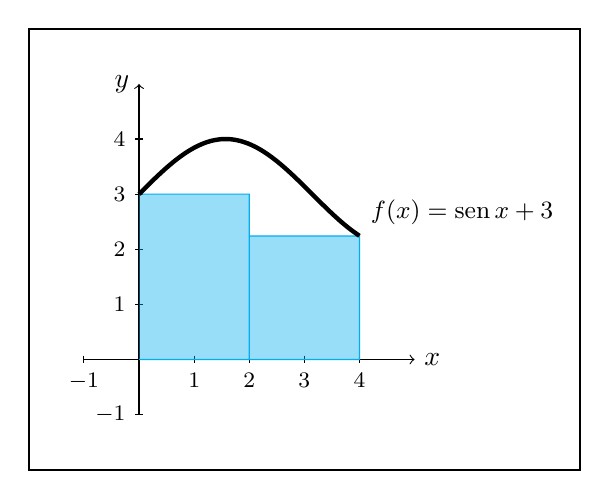
\begin{tikzpicture}[scale=0.7]
			\draw[thick] (-2,-2) rectangle (8, 6);
			% Eixos
			\draw[->] (-1,0) -- (5,0) node[right] {$x$};
			\draw[->] (0,-1) -- (0, 5) node[left] {$y$};
			
			% Rótulos
			\foreach \i in {-1,1,2,3,4}{
				\draw (\i,2pt)--(\i, -2pt) node[below]{{\footnotesize $\i$}};
			}
			
			\foreach \i in {-1,1,2,3,4}{
				\draw (2pt,\i)--(-2pt, \i) node[left]{{\footnotesize $\i$}};
			}
				% Plot do gráfico
			\filldraw[domain=0:2,smooth,variable=\x, cyan, fill opacity=0.4] plot ({\x},{3})--(2,0)--(0,0);
			\filldraw[domain=2:4,smooth,variable=\x, cyan, fill opacity=0.4] plot ({\x},{2.24})--(4,0)--(2,0);	
			
			\draw[domain=0:4,smooth,variable=\x, ultra thick]  plot ({\x},{3+sin(\x r)})  node[above right] {{\small $f(x) = \textrm{sen}\,x + 3$}};
	
		\end{tikzpicture}
		
	}{
		\Fonte{Elaborado pelo autor}
	}   
\end{figure}

\hspace{-2cm} Vamos escolher outra função simples $\phi_4$ tal que $\phi_4 =\sum_{j = 1}^{4} a_j\chi_{E_j}$
onde 
$E_1 = [0, 1),\ 
 E_2 = [1, 2),\ 
 E_3 = [2, 3),\ 
 E_1 = [3, 4],\ 
 a_1 = f(0), \ 
 a_2 = f(1), \ 
 a_3 = f(3)$ e $a_4 = f(4)$.
Desta forma, com o dobro de valores da função $\phi_2$ escolhida anteriormente podemos observar que a integral de $\phi_4$, exibida na figura \ref{fig:integral da função phi 4}, mais se aproxima da integral da função $f$.
\begin{figure}[h!]
	\centering
	\Caption{\label{fig:integral da função phi 4} Integral da função $\phi_4$} 
	\UECEfig{}{
		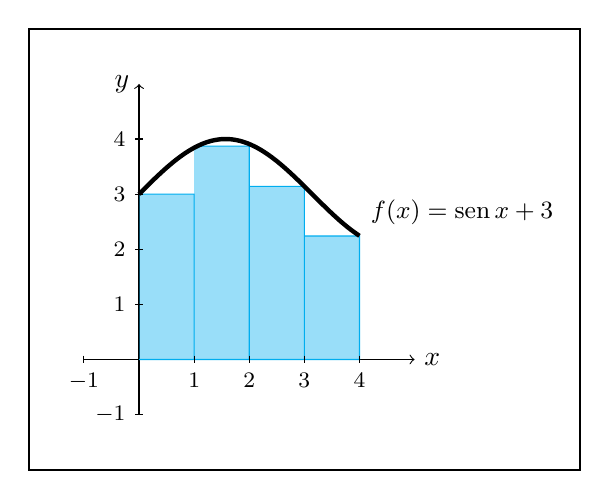
\begin{tikzpicture}[scale=0.7]
			\draw[thick] (-2,-2) rectangle (8, 6);
			% Eixos
			\draw[->] (-1,0) -- (5,0) node[right] {$x$};
			\draw[->] (0,-1) -- (0, 5) node[left] {$y$};
			
			% Plot do gráfico
			\filldraw [domain=0:1,smooth,variable=\x, cyan, fill opacity=0.4]  plot ({\x},{3})--(1,0)--(0,0);
			\filldraw[domain=1:2,smooth,variable=\x, cyan, fill opacity=0.4] plot ({\x},{3.87})--(2,0)--(1,0);	
			\filldraw[domain=2:3,smooth,variable=\x, cyan, fill opacity=0.4] plot ({\x},{3.14})--(3,0)--(2,0);
			\filldraw[domain=3:4,smooth,variable=\x, cyan, fill opacity=0.4] plot ({\x},{2.24})--(4,0)--(3,0);
					
			% Rótulos
			\foreach \i in {-1,1,2,3,4}{
				\draw (\i,2pt)--(\i, -2pt) node[below]{{\footnotesize $\i$}};
			}
			
			\foreach \i in {-1,1,2,3,4}{
				\draw (2pt,\i)--(-2pt, \i) node[left]{{\footnotesize $\i$}};
			}
			
			\draw[domain=0:4,smooth,variable=\x, ultra thick]  plot ({\x},{3+sin(\x r)})  node[above right] {{\small $f(x) = \textrm{sen}\,x + 3$}};
			
		\end{tikzpicture}
		
	}{
		\Fonte{Elaborado pelo autor}
	}   
\end{figure}
Para finalizarmos esta ideia, dobremos a quantidade de valores e escolhamos outra função 
$\phi_8 =\displaystyle\sum_{j = 1}^{8} a_j\chi_{E_j}$ 
onde 
$E_1 = [0, 0.5),\
 E_2 = [0.5, 1),\ 
 E_3 = [1, 1.5),\ 
 E_4 = [1.5, 2),\ 
 E_5 = [2,2.5), \ 
 E_6 = [2.5, 3), \ 
 E_7 = [3, 2.5), \ 
 E_8 = [3.5, 4]$ 
e
$a_1 = f(0),\ 
 a_2 = f(0.5),\ 
 a_3 = f(1), \ 
 a_4 = f(1.5),\ 
 a_5 = f(2.5), \ 
 a_6 = f(3), \ 
 a_7 = f(3.5)$ e $a_8 = f(4)$.
A integral da função $\phi_8$ está representada na figura 
figura \ref{fig:integrla da função phi 8}.
\begin{figure}[h!]
	\centering
	\Caption{\label{fig:integrla da função phi 8} Integral da função $\phi_8$} 
	\UECEfig{}{
		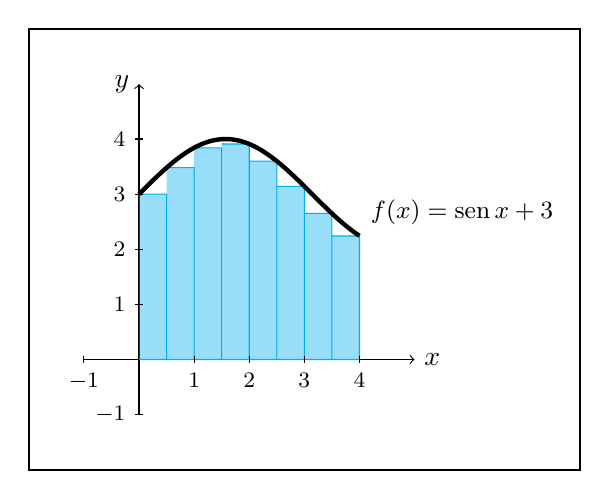
\begin{tikzpicture}[scale=0.7]
			\draw[thick] (-2,-2) rectangle (8, 6);
			% Eixos
			\draw[->] (-1,0) -- (5,0) node[right] {$x$};
			\draw[->] (0,-1) -- (0, 5) node[left] {$y$};
			
			% Plot do gráfico
			\filldraw [domain=0:0.5,smooth,variable=\x, cyan, fill opacity=0.4]  plot ({\x},{3})--(0.5,0)--(0,0);
			
			\filldraw [domain=0.5:1,smooth,variable=\x, cyan, fill opacity=0.4]  plot ({\x},{3.48})--(1,0)--(0.5,0);
			
			\filldraw[domain=1:1.5,smooth,variable=\x, cyan, fill opacity=0.4] plot ({\x},{3.84})--(1.5,0)--(1,0);	
			
			\filldraw[domain=1.5:2,smooth,variable=\x, cyan, fill opacity=0.4] plot ({\x},{3.91})--(2,0)--(1.5,0);
			
			\filldraw[domain=2:2.5,smooth,variable=\x, cyan, fill opacity=0.4] plot ({\x},{3.6})--(2.5,0)--(2,0);
			
			\filldraw[domain=2.5:3,smooth,variable=\x, cyan, fill opacity=0.4] plot ({\x},{3.14})--(3,0)--(2.5,0);
			
			\filldraw[domain=3:3.5,smooth,variable=\x, cyan, fill opacity=0.4] plot ({\x},{2.65})--(3.5,0)--(3,0);
			
			\filldraw[domain=3.5:4,smooth,variable=\x, cyan, fill opacity=0.4] plot ({\x},{2.24})--(4,0)--(3.5,0);
			
			% Rótulos
			\foreach \i in {-1,1,2,3,4}{
				\draw (\i,2pt)--(\i, -2pt) node[below]{{\footnotesize $\i$}};
			}
			
			\foreach \i in {-1,1,2,3,4}{
				\draw (2pt,\i)--(-2pt, \i) node[left]{{\footnotesize $\i$}};
			}
			
			\draw[domain=0:4,smooth,variable=\x, ultra thick]  plot ({\x},{3+sin(\x r)})  node[above right] {{\small $f(x) = \textrm{sen}\,x + 3$}};
			
		\end{tikzpicture}
		
	}{
		\Fonte{Elaborado pelo autor}
	}   
\end{figure}

Com isso, observamos que quanto mais valores a função simples possui, mais ela se aproxima da função $f$ desde que nenhum valor ultrapasse o gráfico da função.
Assim, a área da função simples será próxima o suficiente da área delimitada pelo gráfico da função $f$.
Ou seja, se tomarmos o supremo dessas funções obteremos a integral exposta na figura \ref{fig:Integral da função f}.
\begin{figure}[h!]
	\centering
	\Caption{\label{fig:Integral da função f} Integral da função $f$} 
	\UECEfig{}{
		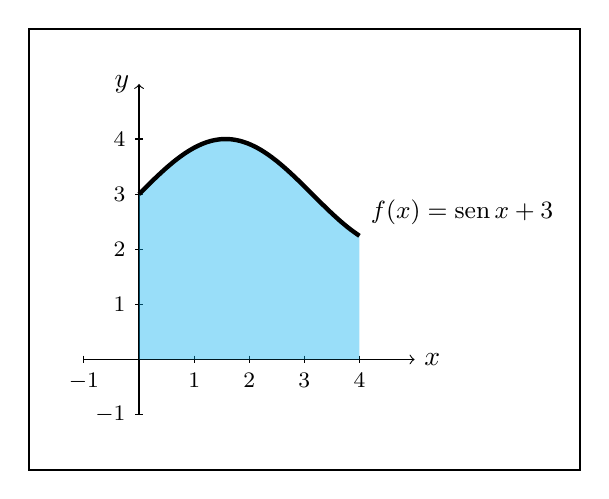
\begin{tikzpicture}[scale=0.7]
			\draw[thick] (-2,-2) rectangle (8, 6);
			% Eixos
			\draw[->] (-1,0) -- (5,0) node[right] {$x$};
			\draw[->] (0,-1) -- (0, 5) node[left] {$y$};
			% Rótulos
			\foreach \i in {-1,1,2,3,4}{
				\draw (\i,2pt)--(\i, -2pt) node[below]{{\footnotesize $\i$}};
			}
			
			\foreach \i in {-1,1,2,3,4}{
				\draw (2pt,\i)--(-2pt, \i) node[left]{{\footnotesize $\i$}};
			}
			\fill[domain=0:4,smooth,variable=\x, cyan, fill opacity=0.4]  plot ({\x},{3+sin(\x r)})--(4,0)--(0,0);
			% Yes, this is drawn twice, but I wanted the shading to match the over/under pictures following.
			
			
			\draw[domain=0:4,smooth,variable=\x, ultra thick]  plot ({\x},{3+sin(\x r)})  node[above right] {{\small $f(x) = \textrm{sen}\,x + 3$}};
		\end{tikzpicture}
		
	}{
		\Fonte{Elaborado pelo autor}
	}   
\end{figure}

Agora, tomemos como exemplo a função $f(x) = x^2$, mas não invés de particionarmos o domínio da função, a função simples é construída conforme uma partição feita na imagem.
Assim, tomemos uma função $\phi_1$ pondo
$$
\phi_1(x) =\left\{
\begin{array}{ll}
	0, & \textrm{se\ } 0 \leq f(x) < 2^{-1} \\
	2^{-1}, & \textrm{se\ } 2^{-1} \leq f(x) < 2\cdot2^{-1} \\
	1, & \textrm{se\ } f(x) \geq 1
\end{array}
\right.
$$

Note que a função $\phi_1$ é simples, mas seus valores são escolhidos por meio da partição da imagem conforme explicitado na imagem da figura \ref{fig: Lebesgue gráfico da função phi 1}.

\begin{figure}[h!]
	\centering
	\Caption{\label{fig: Lebesgue gráfico da função phi 1}Gráfico da função $\phi_1$} 
	\UECEfig{}{
		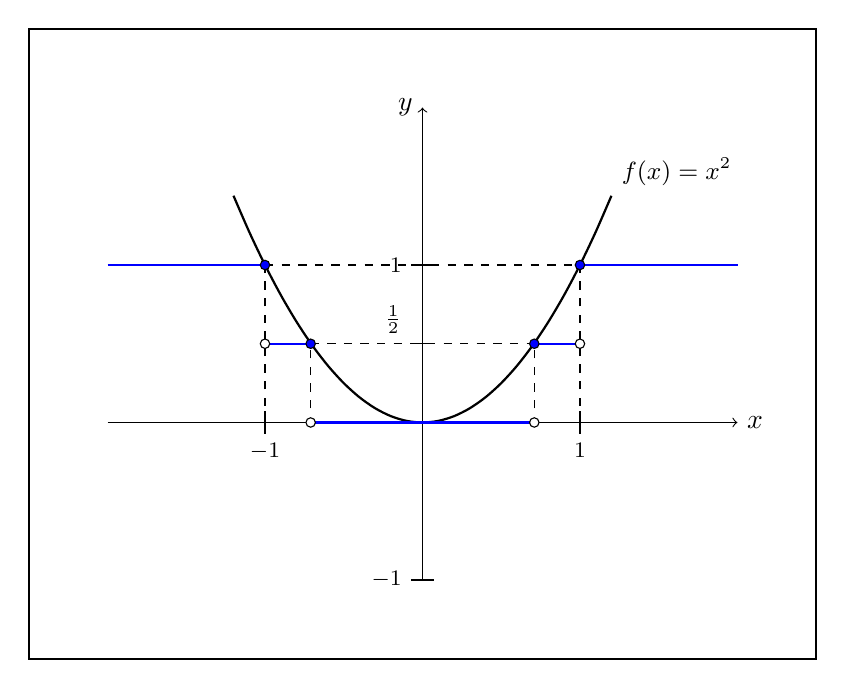
\begin{tikzpicture}[scale=2]
			\draw[thick] (-2.5,-1.5) rectangle (2.5, 2.5);
			% Eixos
			\draw[->] (-2,0) -- (2,0) node[right] {$x$};
			\draw[->] (0,-1) -- (0, 2) node[left] {$y$};
			% Rótulos
			\foreach \i in {-1,1}{
				\draw (\i,2pt)--(\i, -2pt) node[below]{{\footnotesize $\i$}};
			}
			
			\foreach \i in {-1, 1}{
				\draw (2pt,\i)--(-2pt, \i) node[left]{{\footnotesize $\i$}};
			}
			
			\draw (2pt,0.5)--(-2pt, 0.5) node[above left]{\footnotesize $\frac{1}{2}$};
			
			%\fill[domain=-1:1,smooth,variable=\x, cyan, fill opacity=0.4]  plot ({\x},{\x*\x})--(4,0)--(0,0);
			% Yes, this is drawn twice, but I wanted the shading to match the over/under pictures following.
			
			
			\draw[domain=-1.2:1.2,smooth,variable=\x, thick]  plot ({\x},{\x*\x})  node[above right] {{\small $f(x) = x^2$}};
			
			
			% Função $\phi_1$
			\draw[domain=-0.71:0.71,smooth,variable=\x,thick, blue]  plot ({\x},{0});
			
			\draw[domain=-1:-0.71,smooth,variable=\x,thick, blue]  plot ({\x},{0.5});
			\draw[domain=0.71:1,smooth,variable=\x,thick, blue]  plot ({\x},{0.5});
			
			\draw[domain=-2:-1,smooth,variable=\x,thick, blue]  plot ({\x},{1});
			\draw[domain=1:2,smooth,variable=\x,thick, blue]  plot ({\x},{1});
			
			% Retas auxiliares
			\draw[dashed] (-0.71,0.09) -- (-0.71,0.5);
			\draw[dashed] (0.71,0.09) -- (0.71,0.5);
			
			\draw[dashed] (-0.71,0.5) -- (0.71,0.5);
			
			\draw[dashed] (-1,1) -- (1,1);
			
			\draw[dashed] (-1,0) -- (-1,1);
			\draw[dashed] (1,0) -- (1,1);
			
			% Bolinhas
			\draw[fill=white] (-0.71,0) circle (0.03);
			\draw[fill=white] (0.71,0) circle (0.03);
			
			\draw[fill=blue] (-0.71,0.5) circle (0.03);
			\draw[fill=blue] (0.71,0.5) circle (0.03);
			
			\draw[fill=white] (-1,0.5) circle (0.03);
			\draw[fill=white] (1,0.5) circle (0.03);
			
			\draw[fill=blue] (-1,1) circle (0.03);
			\draw[fill=blue] (1,1) circle (0.03);
			
		\end{tikzpicture}
		
	}{
		\Fonte{Elaborado pelo autor}
	}   
\end{figure}

Vamos aproximar a função $f$ agora pela função simples $\phi_2$ construída da seguinte forma:

$$
\phi_2(x) =\left\{
\begin{array}{ll}
	0, & \textrm{se\ } 0 \leq f(x) < 2^{-2} \\
	2^{-2}, & \textrm{se\ } 2^{-2} \leq f(x) < 2\cdot2^{-2} \\
	2\cdot 2^{-2}, & \textrm{se\ } 2\cdot 2^{-2} \leq f(x) < 3\cdot2^{-2}\\
	3\cdot 2^{-2}, & \textrm{se\ } 3\cdot 2^{-2} \leq f(x) < 4\cdot2^{-2}\\
	4\cdot 2^{-2}, & \textrm{se\ } 4\cdot 2^{-2} \leq f(x) < 5\cdot2^{-2}\\
	5\cdot 2^{-2}, & \textrm{se\ } 5\cdot 2^{-2} \leq f(x) < 6\cdot2^{-2}\\
	6\cdot 2^{-2}, & \textrm{se\ } 6\cdot 2^{-2} \leq f(x) < 7\cdot2^{-2}\\
	7\cdot 2^{-2}, & \textrm{se\ } 7\cdot 2^{-2} \leq f(x) < 8\cdot2^{-2}\\
	2, & \textrm{se\ } f(x) \geq 2\\
\end{array}
\right.
$$

Assim, na figura \ref{fig: Lebesgue gráfico da função phi 2} está a comparação com o gráfico da função $f(x) = x^2$.
\begin{figure}[h!]
	\centering
	\Caption{\label{fig: Lebesgue gráfico da função phi 2}Gráfico da função $\phi_1$} 
	\UECEfig{}{
		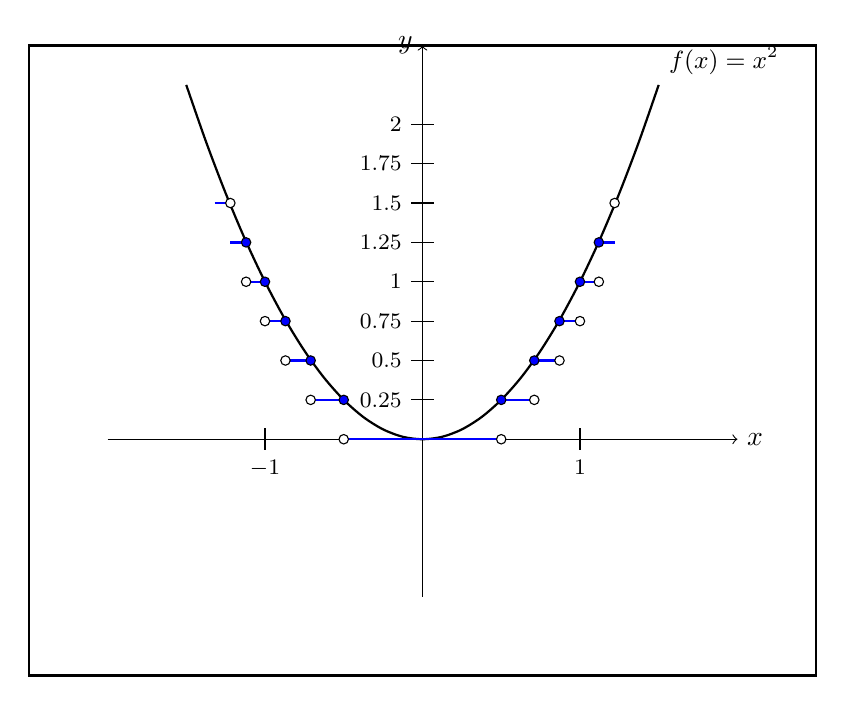
\begin{tikzpicture}[scale=2]
			\draw[thick] (-2.5,-1.5) rectangle (2.5, 2.5);
			% Eixos
			\draw[->] (-2,0) -- (2,0) node[right] {$x$};
			\draw[->] (0,-1) -- (0, 2.5) node[left] {$y$};
			% Rótulos
			\foreach \i in {-1,1}{
				\draw (\i,2pt)--(\i, -2pt) node[below]{{\footnotesize $\i$}};
			}
			
			\foreach \i in {0.25, 0.5, 0.75, 1, 1.25, 1.5,  1.75, 2}{
				\draw (2pt,\i)--(-2pt, \i) node[left]{{\footnotesize $\i$}};
			}
			
		%	\draw (2pt,0.5)--(-2pt, 0.5) node[above left]{\footnotesize $\frac{1}{2}$};
			
			%\fill[domain=-1:1,smooth,variable=\x, cyan, fill opacity=0.4]  plot ({\x},{\x*\x})--(4,0)--(0,0);
			% Yes, this is drawn twice, but I wanted the shading to match the over/under pictures following.
			
			
			\draw[domain=-1.5:1.5,smooth,variable=\x, thick]  plot ({\x},{\x*\x})  node[above right] {{\small $f(x) = x^2$}};
			
			
			% Função $\phi_2$
			\draw[domain=-0.5:0.5,smooth,variable=\x,thick, blue]  plot ({\x},{0});
			
		
			\draw[domain=-0.71:-0.5,smooth,variable=\x,thick, blue]  plot ({\x},{0.25});
			\draw[domain=0.5:0.71,smooth,variable=\x,thick, blue]  plot ({\x},{0.25});
			
			\draw[domain=-0.87:-0.71,smooth,variable=\x,thick, blue]  plot ({\x},{0.5});
			\draw[domain=0.71:0.87,smooth,variable=\x,thick, blue]  plot ({\x},{0.5});
			
			\draw[domain=-1:-0.87,smooth,variable=\x,thick, blue]  plot ({\x},{0.75});
			\draw[domain=0.87:1,smooth,variable=\x,thick, blue]  plot ({\x},{0.75});
						
			\draw[domain=-1.12:-1,smooth,variable=\x,thick, blue]  plot ({\x},{1});
			\draw[domain=1:1.12,smooth,variable=\x,thick, blue]  plot ({\x},{1});
			
			\draw[domain=-1.22:-1.12,smooth,variable=\x,thick, blue]  plot ({\x},{1.25});
			\draw[domain=1.12:1.22,smooth,variable=\x,thick, blue]  plot ({\x},{1.25});
			
			\draw[domain=-1.32:-1.22,smooth,variable=\x,thick, blue]  plot ({\x},{1.5});
			\draw[domain=1.22:1.22,smooth,variable=\x,thick, blue]  plot ({\x},{1.5});
			
			%\draw[domain=-2:-1,smooth,variable=\x,thick, blue]  plot ({\x},{1.75});
			%\draw[domain=1:2,smooth,variable=\x,thick, blue]  plot ({\x},{1.75});
			
			%\draw[domain=-2:-1,smooth,variable=\x,thick, blue]  plot ({\x},{2});
			%\draw[domain=1:2,smooth,variable=\x,thick, blue]  plot ({\x},{2});
			
			% Retas auxiliares
			%\draw[dashed] (-0.71,0.09) -- (-0.71,0.5);
			%\draw[dashed] (0.71,0.09) -- (0.71,0.5);
			
			%\draw[dashed] (-0.71,0.5) -- (0.71,0.5);
			
			%\draw[dashed] (-1,1) -- (1,1);
			
			%\draw[dashed] (-1,0) -- (-1,1);
			%\draw[dashed] (1,0) -- (1,1);
			
			% Bolinhas
			\draw[fill=white] (-0.5,0) circle (0.03);
			\draw[fill=white] (0.5,0) circle (0.03);
			
			\draw[fill=blue] (-0.5, 0.25) circle (0.03);
			\draw[fill=blue] (0.5, 0.25) circle (0.03);
			
			\draw[fill=white] (-0.71,0.25) circle (0.03);
			\draw[fill=white] (0.71,0.25) circle (0.03);
			
			\draw[fill=blue] (-0.71,0.5) circle (0.03);
			\draw[fill=blue] (0.71,0.5) circle (0.03);
			
			\draw[fill=white] (-0.87,0.5) circle (0.03);
			\draw[fill=white] (0.87,0.5) circle (0.03);
			
			\draw[fill=blue] (-0.87,0.75) circle (0.03);
			\draw[fill=blue] (0.87,0.75) circle (0.03);
			
			\draw[fill=white] (-1,0.75) circle (0.03);
			\draw[fill=white] (1,0.75) circle (0.03);
			
			\draw[fill=blue] (-1,1) circle (0.03);
			\draw[fill=blue] (1,1) circle (0.03);
			
			\draw[fill=white] (-1.12,1) circle (0.03);
			\draw[fill=white] (1.12,1) circle (0.03);
			
			\draw[fill=blue] (-1.12,1.25) circle (0.03);
			\draw[fill=blue] (1.12,1.25) circle (0.03);
			
			\draw[fill=white] (-1.22,1.5) circle (0.03);
			\draw[fill=white] (1.22,1.5) circle (0.03);
			
		\end{tikzpicture}
		
	}{
		\Fonte{Elaborado pelo autor}
	}   
\end{figure}

Dito isto, adiante formalizaremos que dada uma função $f \in \menfus$, então ela pode ser aproximada por uma sequência de funções simples conforme o teorema adiante.

\begin{env}{Teorema}[Aproximação Via Funções Simples]
	\label{teo:aproximação via funções simples}
	Se $f$ é uma função não negativa em $\menfus$, então existe uma sequência de funções $(\varphi_n)$ tal que $\phi \in \menfus, \forall \ n \in \N$ de forma que
	\begin{enumerate}[label*=(\roman*)]
		\item Cada $\varphi_n$ é uma função simples, isto é, possui apenas uma quantidade finita de valores reais;
		\item $0 \leq \varphi_n(x) \leq f(x)$ para todo $x \in X$ e $n \in \N$;
		\item $\displaystyle\lim_{n \to \infty} \varphi_n(x) = f(x)$ para todo $x \in X$.
	\end{enumerate}
\end{env} 

\begin{prova}
	Vamos mostrar a existência das sequência por construção.
	Essa construção será realizada por meio de partições da imagem da seguinte maneira:
	
	$$
	\varphi_n(x) =\left\{
	\begin{array}{ll}
		0, & \textrm{se\ } 0 \leq f(x) < 2^{-n} \\
		2^{-n}, & \textrm{se\ } 2^{-n} \leq f(x) < 2\cdot2^{-n} \\
		2\cdot2^{-n}, & \textrm{se\ } 2\cdot2^{-n} \leq f(x) < 3\cdot2^{-n} \\
		\vdots & \vdots \\
		k\cdot2^{-n}, & \textrm{se\ } k\cdot2^{-n} \leq f(x) < (k+1)\cdot2^{-n} \\
		\vdots & \vdots \\
		n, & \textrm{se\ } f(x) \geq n
	\end{array}
	\right.
	$$
	Simplificadamente podemos escrever
	$$
	\varphi_n(x) =\left\{
	\begin{array}{ll}
		k\cdot2^{-n}, & \textrm{se\ } k\cdot2^{-n} \leq f(x) < (k+1)\cdot2^{-n}, \textrm{para } k = 0,1,2, \ldots, n2^n-1 \\
		n, & \textrm{se\ } f(x) \geq n
	\end{array}
	\right.
	$$
	Com isso, podemos ver que $\varphi_n$ é uma função simples e que $0\leq \varphi_n(x)\leq f(x)$. Além disso, $\varphi_n$ é uma mensurável para todo $n \in \N$, pois trata-se de uma sequência de um funções simples.
	Observe que dado $n \in \N$ temos que
	$\phi_n(x) = k2^{-n}$ desde que 
	$k2^{-n} \leq f(x) < (k+1)2^{-n}$.
	Como  $k2^{-n}+2^{-n}$, percebemos que
	$$
	k2^{-n} \leq f(x) < (k+1)2^{-n}
	\Rightarrow
	k2^{-n} \leq f(x) < k2^{-n} + 2^{-n}
	\Rightarrow
	\phi_n(x) \leq f(x) < \phi_n(x) + 2^{-n}.
	$$
	Logo, 
	$$
	\dlim_{n \to +\infty}\phi_n(x)  
	\leq 
	\dlim_{n \to +\infty}f(x) 
	\leq 
	\dlim_{n \to +\infty}\phi_n(x) 
	+ 
	\dlim_{n \to +\infty}2^{-n}.
	$$
	Como $\dlim_{n \to +\infty} f(x) = f(x)$ e 
	$\dlim_{n \to +\infty} 2^{-n} = 0$.
	Segue, pelo teorema do confronto que
	$\dlim_{n \to +\infty} \phi_n(x) = f(x)$.
\end{prova}

Esse teorema nos mostra que dada qualquer função não negativa mensurável, podemos aproximar seus valores por funções simples de maneira que o limite dessa sequência de funções simples convergem para a função que tomamos inicialmente.
Diante disso, nada mais natural que definir a integral de Lebesgue para funções não negativas quaisquer da maneira que segue
\begin{env}{Definição}
	\label{def:integral de uma função qualquer não negativa}
	Se $f \in M^+(X,\cc)$, nós definimos a integral de $f$ com respeito à medida $\mu$ sendo o valor real estendido
	$$
	\int f d\mu = sup \int \varphi d\mu
	$$
	Onde o supremo é sobre todas as funções simples $\varphi \in \menfus$ tal que a condição $0 \leq \varphi \leq f(x)$ para todo $x \in X$. 
\end{env}

\begin{env}{Definição}
	\label{def: integral de uma função não neg com respeito a um conjunto específico}
	Se $f \in \menfus$ e $E \in \cc$, então $f\chi_{E} \in \menfus$ e nós definimos a integral de $f$ sobre o conjunto $E$ com respeito à medida $\mu$ como sendo o número real estendido
	$$
	\int_E f d\mu = \int f\chi_E d\mu
	$$
\end{env}

Agora desejamos realizar operações aritméticas com essa expansão da definição conforme fizemos para a integral de funções simples.
Para tal, precisamos mostrar a monoticidade da integral de funções não negativas tanto à respeito de uma outra função integral quanto à um conjunto.
Isso faremos por meio dos lemas a seguir

\begin{env}{Lema}
	\label{lem:monoticiadade da integral de funções não negativas}
	Se $f$ e $g$ são elementos de $M^+(X,\cc)$ com $f \leq g$, então 
	$$
	\int fd\mu \leq \int g d\mu.
	$$
\end{env}
\begin{prova}
	Se $\varphi$ é uma função simples em $M^+(X,\cc)$ tal que 
	$0 \leq \varphi \leq f$, então $0 \leq \varphi \leq g$, uma vez que $f \leq g$.
	Assim, 
	$\sup_{\varphi leq f} \int\varphi d\mu \leq \int f d\mu$ e
	$\sup_{\varphi leq f} \int\varphi d\mu \leq \int g d\mu$.
	Subtraindo membro à membro temos 
	$$
	0 \leq  \int f d\mu  - \int g d\mu
	\Leftrightarrow
	\int f d\mu \leq \int g d\mu.
	$$
	
\end{prova}
\begin{env}{Lema}
	\label{lem:monoticiadade da integral com conjunto em funções não negativas}
	Se $f$ é um elemento de $M^+(X,\cc)$ e $E,F \in \cc$ com $E \subseteq F$, então 
	$$
	\int_E fd\mu \leq \int_F f d\mu.
	$$
\end{env}
\begin{prova}
	Como $E \subseteq F$, então $chi_E \leq \chi_F$.
	Assim, $fchi_E \leq f\chi_F$.
	Segue, pelo lema anterior que, 
	$$
	\int_E f d\mu 
	=
	\int f\chi_E d\mu
	\leq 
	\int f\chi_F d\mu
	=
	\int_F f d\mu.
	$$
	Portanto, $ \displaystyle 
	\int_E f d\mu 
	=
	\int_F f d\mu.
	$
\end{prova}

\begin{env}{Teorema}[Teorema da Convergência Monótona]
	\label{teo:Convergencia Monótona}
	Se $(f_n)$ é uma sequência monótona crescente de funções não negativas mensuráveis que converge para a $f$, então
	$$
	\int f d\mu = \dlim_{n \to \infty} \int f_n d\mu
	$$
\end{env}
\begin{prova}
	Pelo corolário \ref{cor:convergencia-de-uma-sequencia-mensuravel}, se temos uma sequência de funções mensuráveis que converge para uma função $f$, então $f$ também é mensurável.
	Além disso,
	como $(f_n)$ é crescente, então $f_n \leq f\ \forall n \in \N$.
	Seque, pelo lema \ref{lem:monoticiadade da integral de funções não negativas} que 
	$$
	\int f_n\ d\mu \leq \int f\ d\mu
	$$
	Para todo $n \in \N$.
	Desta maneira, 
	$$
	\dlim_{n \to +\infty}\int f_n d\mu \leq \int f d\mu.
	$$
	Por outro lado, sejam $\alpha \in \R$ tal que $0 < \alpha <1$ e 
	$\varphi$ uma função simples mensurável tal que $0 \leq \varphi \leq f$.
	Tomando $n \in \N$ tais que $f_n(x) \geq \alpha \varphi(x)$, construa
	os conjuntos 
	$$
	A_n =\{x \in ;\ f_n(x) \geq \alpha \varphi(x)\}.
	$$
	Com isso, podemos observar que cada $A_n \in X$, $A_{n} \subseteq A_{n+1}$
	e que $X = \bigcup_{n \in \N}A_n$.
	Desta maneira, usando o lema \ref{lem:monoticiadade da integral com conjunto em funções não negativas} e \ref{lem:monoticiadade da integral de funções não negativas} temos que 
	\begin{equation}
		\label{eq:desigualdade da volta}
		\int_{A_n} \alpha\varphi d\mu
		\leq
		\int_{A_n} f_n d\mu
		\leq
		\int f_n d\mu.		
	\end{equation}
	Como $(A_n)$ é uma sequência monótona crescente que a união é igual ao conjunto $X$, observamos que, pela proposição \ref{prop:limite-sequencia-crescente} que para uma medida $\mu$ vale
	$$
	\mu(X) = \mu\left(\bigcup_{n \in \N}A_n\right) = \lim_{n \to +\infty} \mu(A_n)
	$$
	Só que pelo teorema \ref{teo:medida-atraves-de-uma-integral} $\int \varphi \chi_E d\mu$ é uma medida.
	Desta forma, 
	$$
	\dlim_{n \to +\infty} \int_{A_n} \varphi d\mu 
	= \dlim_{n \to +\infty} \int \varphi \chi_{A_n} d\mu
	= \int \varphi \chi_X d\mu
	= \int \varphi d\mu.
	$$
	Substituindo isso na equação \ref{eq:desigualdade da volta} obtemos
	$$
	\alpha \int \varphi d\mu \leq \dlim_{n \to +\infty} \int f_n d\mu.
	$$
	Como $\alpha \in (0,1)$ segue que
	$$
	\int \varphi d\mu \leq \dlim_{n \to +\infty} \int f_n d\mu.
	$$
	Finalmente, por $\varphi$ ser uma função não negativa simples arbitrária que satisfaz $0\leq \varphi \leq f$, obtemos
	$$
	\int f d\mu 
	= \sup_{\varphi} \int \varphi d\mu \leq \dlim_{n \to +\infty}\int f_n d\mu.
	$$
	Disso tudo,
	$$
	\int f d\mu 
	\leq 
	\dlim_{n \to +\infty}\int f_n d\mu
	\leq
	\int f d\mu.
	$$
	Portanto,  $\displaystyle \dlim_{n \to +\infty}\int f_n d\mu
	=
	\int f d\mu$ como desejávamos.
\end{prova}

O teorema anterior nos permite mostrar as operações aritméticas para integral de Lebesgue para funções não negativas quaisquer como apresentaremos adiante.

\begin{env}{Corolário}
	Se $f \in M^+$ e $c \geq 0$, então $cf \in M^+$ e vale
	$$
	\int cf d\mu = c\int f d\mu.
	$$
\end{env}


\begin{prova}
	Se o número real for zero, então o resultado sai de forma imediata.
	Suponha que $c > 0$. 
	Assim, pelo teorema \ref{teo:aproximação via funções simples}, existe uma sequência de funções simples $(\varphi_n) \subset M^+$ que converge para a função $f$.
	Logo, a sequência $(c\varphi_n)$ converge para $cf$.
	Desta forma, ao aplicarmos os teoremas \ref{teo:aritmetica-com-integrais-de-funções-simples} e 
	\ref{teo:Convergencia Monótona}, obtemos
	$$
	\int c f d\mu 
	= \dlim_{n \to +\infty} \int c\varphi_n d\mu 
	= \dlim_{n \to +\infty}\left( c\cdot \int \varphi_n d\mu\right)
	= c\cdot \left(\dlim_{n \to +\infty} \int \varphi_n d\mu\right)
	= c \int f d\mu.
	$$
	Como queríamos demonstrar.
\end{prova}


\begin{env}{Corolário}
	\label{cor:soma de integrais de funções não negativas}
	Se $f, g \in M^+$, então $f + g \in M^+$ e vale
	$$
	\int (f + g) d\mu = \int f d\mu + \int g d\mu.
	$$ 	
\end{env}

\begin{prova}
	Analogamente ao corolário anterior, tomemos duas sequências de funções simples $(\varphi_n)$ e $(\psi_n)$ ambas monótonas e crescentes tal que convergem, respectivamente, para $f$ e $g$.
	Segue, pelos teoremas \ref{teo:aritmetica-com-integrais-de-funções-simples} e 
	\ref{teo:Convergencia Monótona} que
	$$
	\int(f+ g) d\mu
	= \dlim_{n \to +\infty} \int (\varphi_n +\psi_n) d\mu
	= \dlim_{n \to +\infty}\int \varphi_nd\mu + \dlim_{n \to +\infty} \int \psi_n d\mu
	= \int f d\mu + \int g d\mu.
	$$
\end{prova}

Note que os resultados tratam apenas de funções monótonas e nem sempre teremos essa condição \enquote{perfeita} para nossas sequências.
Assim, o próximo resultado nos apresenta uma maneira de trabalhar com sequências que não são monótonas.

\begin{env}{Teorema}[Lema de Fatou]
	\label{teo:lema de fatou}
	Se $(f_n) \subset M^+(X, \cc)$, então 
	$\displaystyle
	\int(\lim \inf f_n)d\mu \leq \lim \inf \int f_n d\mu$. 
\end{env}
\begin{prova}
	Tome a sequência $g_m = \inf_{n \in \N}\{f_m, f_{m+1},...\}$.
	Assim, enquanto $m\leq n$ nós temos $g_m \leq f_n$.
	Neste caso,
	$$
	\int g_m d\mu \leq \int f_n d\mu.
	$$
	Como $(g_m)$ é crescente e converge para $\lim\inf f_n$ nós temos que 
	$$
	\int g_m d\mu \leq \lim \inf \int f_n d\mu.
	$$
	Logo, pelo Teorema da Convergência Uniforme,
	$$
	\int (\lim \inf f_n)d\mu = \lim \int g_m d\mu \leq \lim \inf \int f_n d\mu.
	$$ 
\end{prova}

\begin{env}{Corolário}
	Se $f \in M^+$ e $\lambda$ é definida sobre $\cc$ pondo
	$
	\lambda(E) = \int_E fd\mu 
	$,
	então $\lambda$ é uma medida.
\end{env}

\begin{prova}
	Uma vez que $f \geq 0$, obtemos que $\lambda(E) \geq 0$, por definição.
	Caso $E = \varnothing$, então $f\chi_E \equiv 0$ acarretando que $\lambda(\varnothing) = 0$.
	Por fim, tome $(E_n)$ uma sequência disjunta do conjunto $\cc$ e defina
	$f_n$ pondo
	$$
	f_n = \sum_{k =1}^nf\chi_{E_k}
	$$
	Segue do corolário \ref{cor:soma de integrais de funções não negativas} que
	$$
	\int f_n d\mu
	= \int \left(\sum_{k =1}^nf\chi_{E_k}\right) d\mu
	= \sum_{k =1}^n \left(\int f\chi_{E_k}\right) d\mu
	= \sum_{k =1}^n \left(\int_{E_k} f\right) d\mu
	= \sum_{k =1}^n \lambda(E_k) d\mu
	$$
\end{prova}

%%%%%%%%% Definir QUASE TODO PONTO

\begin{env}{Definição}
	\label{def:quase-todo-ponto}
	Diremos que alguma propriedade ocorre em quase todo ponto de um conjunto $X$ com respeito à medida $\mu$, se ela não é valida somente em um subconjunto $E$ de $X$ que tem medida nula.
	Denotaremos esse acontecimento por $\mu$-q.t.p.
\end{env}

\begin{env}{Corolário}
	Suponha que $f \in M^+$. Então
	$f(x) = 0$ em quase todo ponto de $X$ se, e somente se $\displaystyle \int fd\mu = 0$.
\end{env}

\begin{prova}
	Suponha $f(x) = 0$ $\mu$-q.t.p.
	Assim, se $E = \{ x \in X: f(x) > 0\}$, então $\mu(E) = 0$.
	Tome a sequência $f_n = n\chi_E$.
	Dessa forma $f \leq \lim \inf_{n \in \N} f_n$.
	Segue, pelo Lema de Fatou que
	$$
	0 
	\leq
	\int f d\mu
	\leq
	\int (\lim \inf f_n) d\mu
	\leq
	\lim \inf \int f_n d\mu
	=
	0.
	$$
	Ou seja, $\displaystyle\int f d\mu = 0$.
	Reciprocamente, suponha que $\displaystyle\int f d\mu = 0$.
	Tome uma sequência de conjuntos 
	$E_n = \left\{ x \in X. f(x) > \dfrac{1}{n}\right\}$ tal que 
	$f \geq \left(\dfrac{1}{n}\right)\chi_{E_n}$.
	Assim, $\int f d\mu \geq \int \left(\dfrac{1}{n}\right)\chi_{E_n} d\mu$.
	Só que 
	$\int \left(\dfrac{1}{n}\right)\chi_{E_n} d\mu
	= \dfrac{1}{n}\mu(E_n) \geq 0.
	$
	Segue que
	$$
	0 = \inf f d\mu 
	\geq 
	\dfrac{1}{n}\mu(E_n) \geq 0
	$$
	Ou seja $\mu(E_n) = 0$ para todo $n \in \N$.
	Assim, todo $E_n$ tem medida nula.
	Segue, pela proposição \ref{prop:medida-nula-união}
	que o conjunto $\{x \in X; f(x) > 0\}$ tem medida nula, pois
	$\{x \in X; f(x) > 0\}
	=
	\displaystyle
	\bigcup_{n \in \N} E_n.
	$
	
\end{prova}
Finalizaremos esta subseção apresentando um corolário do Teorema da Convergência Monótona que enfatiza claramente a diferença entre a Integral de Riemann e a Integral de Lebesgue.

\begin{env}{Corolário}
	Se $(g_n)$ é uma sequência de funções em $M^+$, então 
	$$
	\int \left(\dsum_{n = 1} ^\infty g_n\right)d\mu
	=
	\dsum_{n = 1} ^\infty \left(\int g_n d\mu\right).
	$$
\end{env}
\begin{prova}
	O resultado sai imediatamente da aplicação do Teorema da Convergência Monótona considerando a sequência de funções $(f_n) \subset M^+$ tais que
	$f_n = g_1 + \cdots + g_n  $.
\end{prova}
\section{Funções Integráveis}
Definimos anteriormente apenas integrais de funções não negativas com respeito à uma medida $\mu$.
Nesta estenderemos, finalmente, este conceito para uma função qualquer de valores reais estendidos. Com isso,

\begin{env}{Definição}
	Seja $L = (X, \cc, \mu)$ a coleção de funções integráveis que consiste de todas as funções reais $\cc$-mensuráveis $f:X \to \R$ tais que as funções
	$f^+$ e $f^-$ são ambas integrais finitas com respeito à medida $\mu$.
	Neste caso, nós definimos a integral de $f$ com respeito à medida $\mu$ como
	$$
	\int fd\mu
	= \int f^+ d\mu - \int f^- d\mu
	$$
	Se, por ventura, $E$ for um elemento da \sigal $\cc$, então definimos
	$$
	\int_E fd\mu
	= \int_E f^+ d\mu - \int_E f^- d\mu
	$$
\end{env}

\begin{env}{Teorema}
	\label{teo:f é integrável se, só, se |f| o é}
	Uma função mensurável $f$ é um elemento de $L$ se, e somente se, $|f|$ é um elemento de $L$.
\end{env}

\begin{prova}
	Suponha que $f \in L$.
	Por definição, isso ocorre se, e somente se, as artes positiva e negativa de $f$ são ambas elementos de $M^+$ e suas, respectivas integrais, são finitas.
	Devemos mostrar que 
	$$
		\int |f| d\mu = \int |f|^+ d\mu - \int |f|^-d\mu
	$$
	Pela definição \ref{def:parte-positiva e negativa}, $|f|^- = 0$, logo 
	$\int |f|^- d\mu = 0$.
	Pelo lema \ref{lem:decomposicao-da-funcao-em-partes-positiva-negativa} temos que
	$|f|^+ = |f| = f^+ + f^-$.
	Assim, $\displaystyle \int |f|^+ d\mu = \int (f^+ + f^-)d\mu$.
	Como $f^+ + f^- \in M^+$, segue pelo corolário \ref{cor:soma de integrais de funções não negativas} que 
	$\displaystyle\int (f^+ + f^-)d\mu = \int f^+ d\mu + \int f^- d\mu$, ou seja $\displaystyle\int |f|^+d\mu$ é finita.
	Desta forma, 
	$$
	\int |f| d\mu 
	= \int (f^+ + f^-)d\mu - 0 
	= \int |f|^+ d\mu - \int |f|^- d\mu
	$$
	Logo, $|f| \in L$.
	A recíproca é totalmente análoga.	
\end{prova}

\begin{env}{Corolário}
	Se $|f| \in L$, então $\displaystyle \left|\int f d\mu\right| \leq \int |f| d\mu$.
\end{env}
\begin{prova}
	Se $|f| \in L$, então $f \in L$ pelo teorema anterior.
	Logo $\int f^+ d\mu$ e $\int f^- d\mu$ são finitas e não negativas.
	Desta forma
	\begin{align*}
		\left|\int f d\mu \right|
		=
		\left|\int f^+ d\mu - \int f^- d\mu\right|
		= &
		\left|\int f^+ d\mu + \left(- \int f^- d\mu\right)\right|\\
		\leq&
		\left|\int f^+ d\mu\right| + \left|\left(- \int f^- d\mu\right)\right|\\
		=&
		\int f^+ d\mu + \int f^- d\mu\\
		= &
		\int (f^+ + f^-) d\mu\\
		=&¨
		\int |f| d\mu.
	\end{align*}
	Portanto, $\displaystyle \left|\int f d\mu \right| \leq  \int |f| d\mu.$
\end{prova}

\begin{env}{Corolário}
	\label{cor: f é mensurável, g é integrável então f é integrável}
	Se $f$ é mensurável, $g$ é integrável e $|f| \leq |g|$, então  $f$ é integrável e $\displaystyle \int |f| d\mu \leq \int |g| d\mu$.
\end{env}
\begin{prova}
	Se $f$ é mensurável, então para uma medida $\mu$ definida sobre $(X,\cc)$, tem-se que $f \in L$. Assim, pelo teorema \ref{teo:f é integrável se, só, se |f| o é} tem-se que $|f|$ é integrável.
	Como $|f|$ e $|g|$ são função não negativas, segue pelo lema
	\ref{lem:monoticiadade da integral de funções não negativas} que 
	$\displaystyle \int |f| d\mu \leq \int |g| d\mu$.
\end{prova}


\begin{env}{Teorema}
	\label{teo: soma e multiplicação por escalar de funções integráveis}
	Se $f, g \in L$ e $\alpha \in \R$. Então
	\begin{enumerate}[label*=(\alph*)]
		\item A multiplicação por escalar $\alpha f \in L$ com $\displaystyle \int \alpha fd\mu = \alpha \int f d\mu$;
		\item A soma $(f + g) \in L$ com $\displaystyle \int (f + g) d\mu = \int f d\mu + \int g d\mu$. 
	\end{enumerate}
\end{env}
\begin{prova}
	\begin{enumerate}[label*=(\alph*)]
	\item Se $\alpha = 0$, então $\alpha f = 0$ em todo ponto de seu domínio.
	Assim,
	$
	\displaystyle\int \alpha f d\mu = 0 = \alpha \int f d\mu.
	$
	Se $\alpha > 0$, então 
	\begin{align*}
		\alpha \int f d\mu
		=&	
		\alpha \left( \int f^+ d\mu - \int f^- d\mu\right)\\
		=&
		\alpha\int f^+ d\mu - \alpha\int f^- d\mu\\
		=&
		\int\alpha f^+ d\mu - \int\alpha f^- d\mu.
	\end{align*}
	Perceba que $\alpha f^+ = (\alpha f)^+$  e $\alpha f^- = (\alpha f)^-$.
	Disso, 
	$$
	\int\alpha f^+ d\mu - \int\alpha f^- d\mu
	=
	\int(\alpha f)^+ d\mu - \int(\alpha f)^- d\mu
	=
	\int \alpha f d\mu.
	$$
	Neste caso, $\alpha f \in L$ e temos $\displaystyle \alpha \int f d\mu = \int \alpha f d\mu$. O caso $\alpha < 0$ é totalmente análogo.
	
	\item Se $f, g \in L$, então $|f|,|g| \in L$ pelo teorema \ref{teo:f é integrável se, só, se |f| o é}.
	Como $|f + g| \leq |f| + |g|$, segue que $f + g \in L$ pelo corolário \ref{cor: f é mensurável, g é integrável então f é integrável}.
	Além disso, pelo lema \ref{lem:f = f^+ - f^-}, temos 
	$f = f^+ - f^-$ e $g = g^+ - g^-$.
	Somando membro a membro, temos
	$$
	f + g = f^+ - f^-  + g^+ - g^- = f^+ + g^+ - (f^- + g^-) 
	$$
	Como $(f^+ + g^+), (f^- + g^-)$ são funções integráveis não negativas, temos que 
	$$
	\int (f + g) d\mu =  \int [f^+ + g^+ - (f^- + g^-)] d\mu 
	$$
	Pelo corolário \ref{cor:soma de integrais de funções não negativas} 
	\begin{align*}
		\int [f^+ + g^+ - (f^- + g^-)] d\mu 
		=&
		\int (f^+ + g^+)d\mu - \int(f^- + g^-) d\mu\\
		=&
		\int f^+ d\mu + \int g^+ d\mu - \int f^-d\mu - \int g^- d\mu\\
		=&
		\int f^+ d\mu - \int f^-d\mu + \int g^+ d\mu  - \int g^- d\mu\\
		=&
		\int f d\mu + \int g d\mu.
	\end{align*}
	Portanto, $\displaystyle \int (f+g)d\mu = \int f d\mu + \int g d\mu.$
	\end{enumerate}
\end{prova}

\begin{env}{Teorema}[Teorema da Convergência Dominada de Lebesgue]
	Seja $(f_n)$ uma sequência de funções integráveis que converge em quase todo ponto para uma uma função real mensurável $f$.
	Se existir uma função integrável $g$ tal que $|f_n| \leq g$ para todo $n \in \N$, então $f$ é integrável e $\displaystyle \int f d\mu = \dlim_{n \to +\infty} \int f_n d\mu$.
\end{env}

\begin{prova}
	Se $(f_n)$ converge em quase todo ponto para a função $f$ e $|f_n| \leq g$ para cada $n \in \N$, então $f \leq g$ em quase todo ponto.
	Como $g$ é integrável, segue pelo corolário \ref{cor: f é mensurável, g é integrável então f é integrável} que $f$ é integrável.
	Além disso, note que para todo $n \in \N$, temos
	
	$$
	|f_n| \leq g 
	\Leftrightarrow 
	f_n \leq g 
	\textrm{\ ou \ }
	 f_n \leq -g
	\Leftrightarrow
	g - f_n \geq 0
	\textrm{\ ou \ }
	g + f_n \geq 0
	$$
	Caso tenhamos $g + f_n \geq 0$ podemos utilizar o Lema de Fatou e o teorema \ref{teo: soma e multiplicação por escalar de funções integráveis} de forma que 
	
	\begin{align*}
		\int g d\mu + \int f d\mu =& \int (g + f) d\mu \\
		\leq & \lim \inf \int (g + f_n) d\mu \\
		=& \lim \inf \left(\int g d\mu + \int f_n d\mu\right)\\
		=& \int g d\mu + \lim \inf \int f_n d\mu
	\end{align*}
	isso acarreta que 
	$$
	\int g d\mu + \int f d\mu = \int g d\mu + \lim \inf \int f_n d\mu.
	$$
	Logo, $\displaystyle \int f d\mu \leq \lim \inf \int f_n d\mu$.
	
	Caso ocorra $g - f_n \geq 0$, aplicamos novamente o Lema de Fatou e o teorema \ref{teo: soma e multiplicação por escalar de funções integráveis}.
	Assim, 
	\begin{align*}
		\int g d\mu - \int f d\mu = \int (g - f) d\mu
		\leq  \lim \inf \int (g - f_n) d\mu
		\leq \int g d\mu + \lim \inf \int (- f_n) d\mu.
	\end{align*}
	Lembre que $\displaystyle \lim \inf \int (- f_n) d\mu = - \lim \sup \int f_n d\mu$.
	Com isso, 
	$$
	\int g d\mu - \int f d\mu \leq 
	\int g d\mu + \lim \inf \int (- f_n) d\mu
	=
	\int g d\mu - \lim \sup \int f_n d\mu.
	$$
	Desta forma, $\displaystyle \int f d\mu \geq \lim \sup \int f_n d\mu$.
	Disso tudo, observamos que 
	$$
	\lim \sup \int f_n d\mu \leq  \int f d\mu \leq \lim \inf \int f_n d\mu. 
	$$
	Portanto, $\displaystyle \lim \int f_n d\mu =  \int f d\mu $.
\end{prova}























